%!TEX root = ../../master.tex
\section{Inter-Service Communication}
In the previous section, we described the three core application layer architectural styles. We now turn the focus toward the microservice architecture style and describe some of the possibilities of inter-service communication. One of first decisions, an architect of microservice oriented architectures has to make, is whether communication between services should be \textit{synchronous} or \textit{asynchronous}. \\

\noindent
Synchronous communication refers to calls made to a remote server, which blocks the caller until the operation completes. Synchronous calls are usually implemented using the \textit{request/response} communication style. The essence of request/response is that the caller makes a request and waits for the response. \\

\noindent
Asynchronous communication refers to calls made to a remote server, where \textit{"the caller does not wait for the operation to complete before returning"} \cite[p. 42]{newman2015building}. Asynchronous calls are usually implemented using event-based communication styles. With an event-based communication style, the communication path is inverted.  Newman describes it as, \textit{"instead of client initiating a request asking for things to be done, it instead says this thing happened and expects other parties to know what to do."} \cite[p. 43]{newman2015building}. \\

\noindent
Newman describes a benefit of synchronous communication \textit{"Synchronous communication can be easier to reason about. We know when things have completed successfully or not."} \cite[p. 42]{newman2015building}.
Bonér, CTO at Lightbend, published in March 2016 \textit{Reactive Microservices Architecture} as a proclamation for a more reactive asynchronous communication style. He describes \textit{"REST is widely considered as the default microservice communication protocol. It's important to understand that REST is most often synchronous which makes it a very unfitting default protocol for inter-service communication"} \cite[p. 21]{boner2016reactive}. Bonér further describes the benefits of an asynchronous communication style as services being decoupled in time and space. \\


\noindent As the complexities in the business processes flow increase, management across the boundary of the individual services becomes hard to grasp. Two possible choices to handle these problems are: \textit{Choreography} \cite[p. 45]{newman2015building} and \textit{Orchestration} \cite[p. 44]{newman2015building}.


\begin{figure}[H]%
    \centering
    \subfloat[Orchestration]{{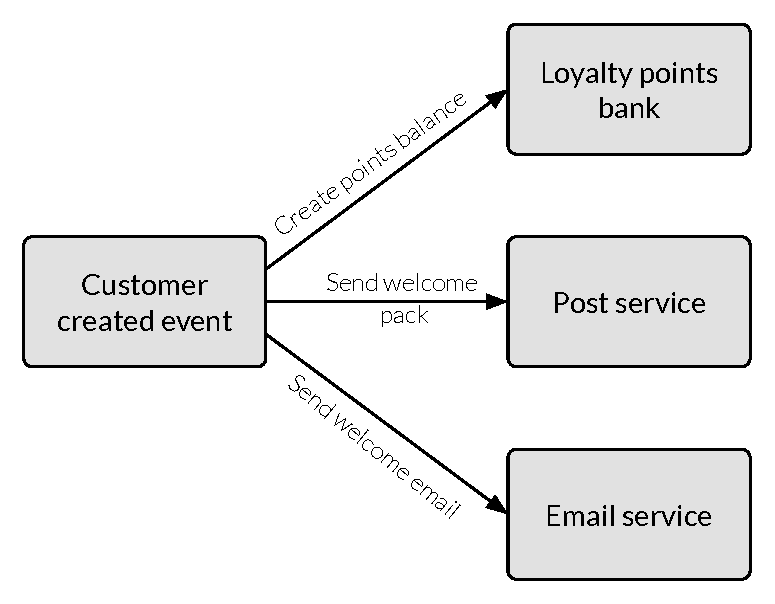
\includegraphics[width=6cm]{figures/orchestration} }}%
    \qquad
    \subfloat[Choreography]{{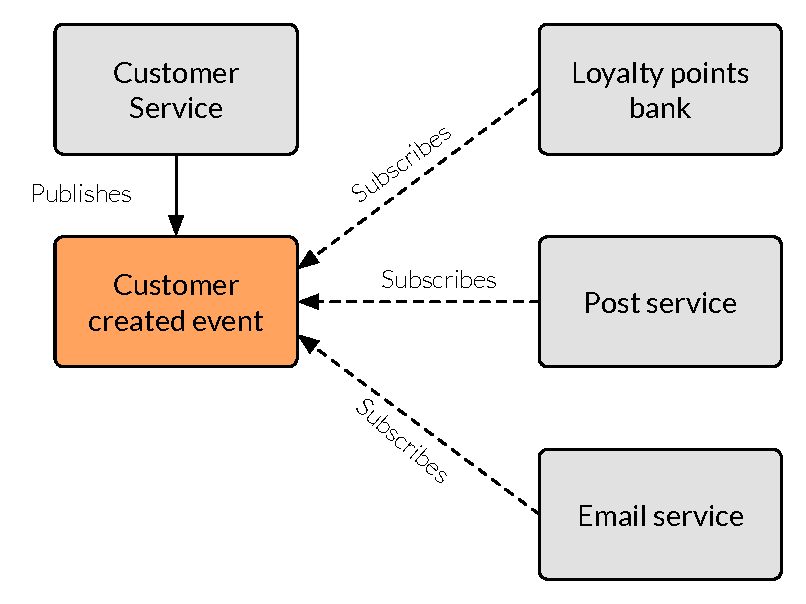
\includegraphics[width=6cm]{figures/choreography} }}%
    \caption{Orchestration Versus Choreography}%
    \label{fig:orch_chor}%
\end{figure}

\subsection*{Orchestration}
Orchestration relies on a single central point to guide and drive the process in the implementation. This central point informs each part of the system of its job and lets it work out the details. In Figure~\ref{fig:orch_chor} (a) an example of orchestration is shown. The Customer service interacts with its services in a synchronous request/response communication style. It is easy for the Customer service to determine whether or not each dependent service has completed its task. A downside to this approach is that the Customer service potentially can become a central governing authority - which is not desirable in a microservice architecture.


\subsection*{Choreography}
Choreography is an asynchronous event-based approach where the customer service emits an event: \textit{Customer created}. The three services know exactly how to respond to this type of event. This results in a much more decoupled architecture, where services instead subscribe to events like in a usual \textit{publish/subscribe} approach. The downsides are that the overall view gets harder to understand and reason about, because of the implicit nature of the architecture. The choreography approach is visualized in Figure~\ref{fig:orch_chor} (b).
Overall, according to Newman: \textit{"systems that tend to be more toward choreographed approach are more loosely coupled, and more flexible and amendable to change"} \cite[p. 45]{newman2015building}.